\documentclass[10pt]{article}
\usepackage[usenames]{color} %used for font color
\usepackage{amssymb} %maths
\usepackage{amsmath} %maths
\usepackage[ruled,linesnumbered]{algorithm2e}
\usepackage[utf8]{inputenc} %useful to type directly diacritic characters

\usepackage{graphics}
\usepackage{adjustbox}
\usepackage{float}
\begin{document}
Stage 4 - User Interface \\\\
\begin{itemize} 

\item{\bf Section 1: Edit Distance Similarity Search UI} 
\textnormal{
The UI for finding semantic similar tweets based on Edit Distance integrated Word2Vec (EDW) and K-medoids clustering (implemented by Lingfei Zeng).\\\\
The mode of user interaction with the data is text queries and mouse clicks. There are two input boxes. The first one is for text input such as a tweet, some key word or a topic (such as hashtags in tweets). The second one is for an integer to indicate how many (top) similar tweets one would like to display. Then mouse click for submit, the UI will return the output, which are the similar tweets. \\\\
The initial UI screenshot in shown Figure \ref{fig1}. After input a tweet and the number of tweets one like to show, the result is shown in Figure \ref{fig2} and Figure \ref{fig3} . One can also input one word as topic or hashtags in the tweets. The search result is shown in  Figure \ref{fig4}. Overall, the output is quite accurate, which indicates the good performance and versatility of our algorithm. \\\\
The error massage will pop out if user does not input anything but hit submit button. It's shown in Figure \ref{fig5}.   
}

 
\begin{figure}[H]
	\caption{Initial UI screen shot}
	\centering
	
\includegraphics[scale=0.3]{Screen_Shot_1.png}
	\label{fig1}
\end{figure}

\begin{figure}[h]
	\caption{Output after input of a tweet}
	\centering
	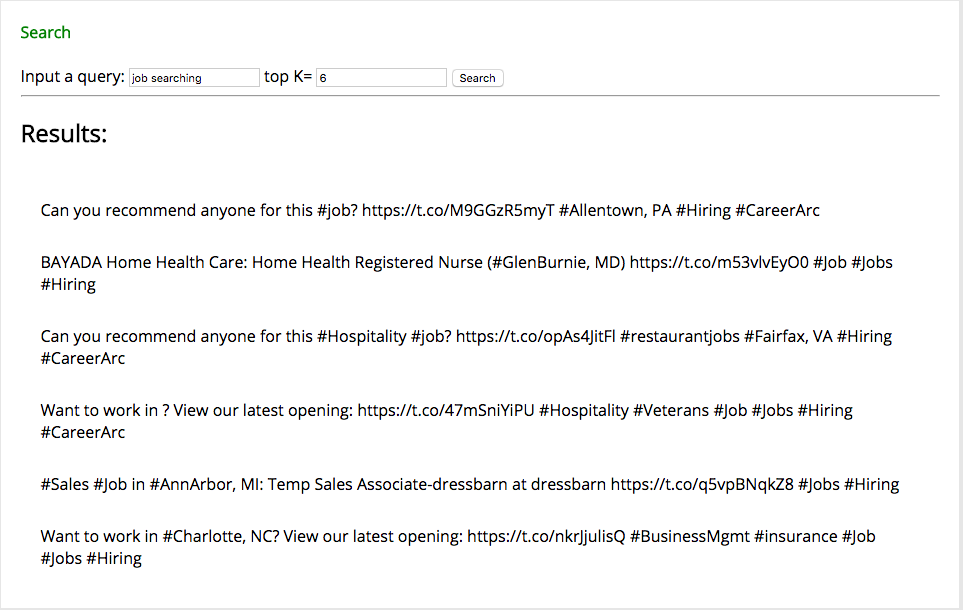
\includegraphics[scale=0.3]{Screen_Shot_2.png}
	\label{fig2}
\end{figure}

\begin{figure}[H]
	\caption{Output after another tweet}
	\centering
	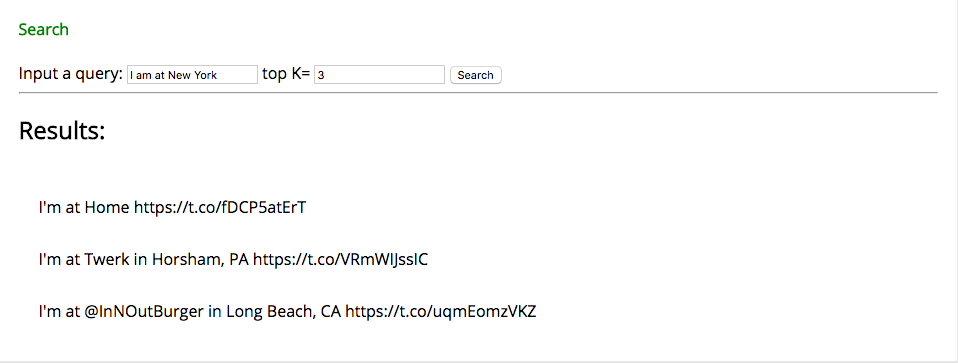
\includegraphics[scale=0.3]{Screen_Shot_3.png}
	\label{fig3}
\end{figure}

\begin{figure}[H]
	\caption{Output after input a hashtag}
	\centering
	\includegraphics[scale=0.3]{Screen_Shot_4.png}
	\label{fig4}
\end{figure}

\begin{figure}[H]
	\caption{Error message when user doesn't input query but hit the submit button }
	\centering
	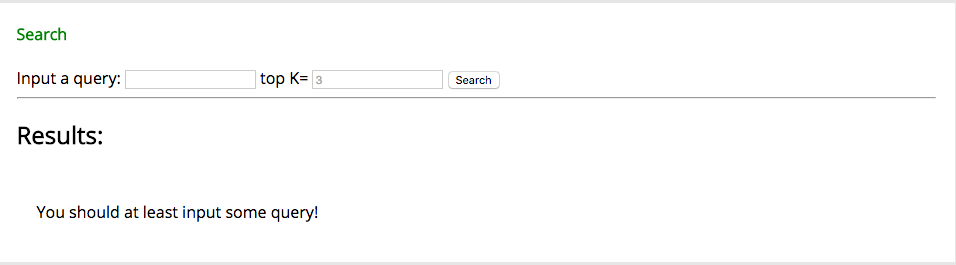
\includegraphics[scale=0.3]{Screen_Shot_5.png}
	\label{fig5}
\end{figure}

\item{\bf Section 3: Network Similarity Search UI} 
\\\\
The Network Similarity Search UI was written in the Python Tkinter library. When the UI starts, it loads the following from the initial dataset: its graph, tweet and hashtag IDs, and scores. 
\\\\
The UI (started by running: run\_UI.py) can be found on: \\
https://github.com/circlefive05/SimRank-on-Twitter-UI
\\\\
A 3 minute demo of the user functions and exception handling cases can be found here: https://youtu.be/CHiQ8C7cdtg
\\\\
\begin{figure}[H]
	\caption{SimRank UI: Search by Tweet }
	\centering
	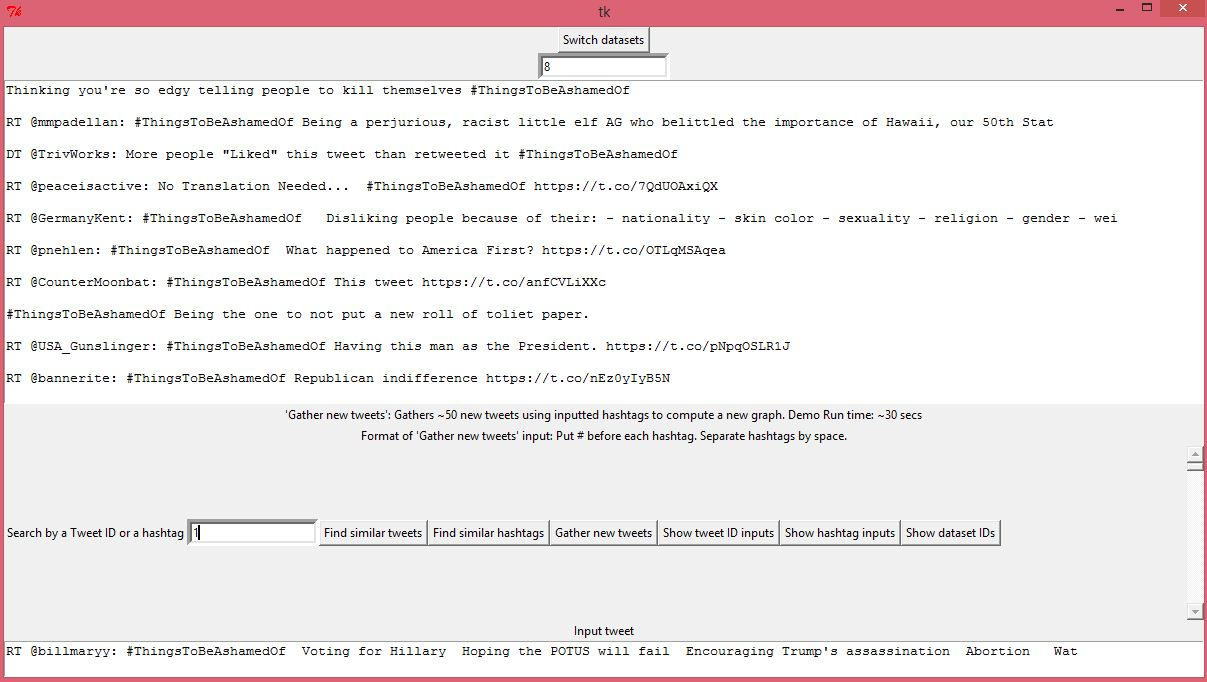
\includegraphics[scale=0.3]{simrank_demo_1.png}
	\label{fig6}
\end{figure}
User functions:
\begin{itemize} 
\item Input tweet and search for similar tweets or hashtags
\item Input hashtag and search for similar tweets or hashtags (different from the input)
\item Input a set of new hashtags, search for new tweets, and return similar tweets or hashtags. Add the newly searched dataset of scores to set of dataset IDs
\item Show tweet IDs in current dataset
\item Show hashtags in current dataset
\item Show current dataset IDs
\item Switch datasets by inputting ID
\end{itemize}

UI displays:
\begin{itemize} 
\item Tweet IDs and hashtags in current dataset
\item If user inputs tweet ID, UI displays both the content of that tweet ID and the similar tweets or hashtags
\item Similar hashtags/tweets
\item Set of dataset IDs
\end{itemize}

Exception Handling- Returns error message on UI if user performs:
\begin{itemize} 
\item If type is integer that is not in current dataset
\item If type in hashtag not in current dataset
\item If, in switching dataset, input is not a valid dataset number
\item If type in hashtag with spaces and don’t search ‘Gather new tweets’
\item If no similar tweets/hashtags found
\item If similar tweets/hashtags found but no new tweets/hashtags found
\end{itemize}

\end{itemize}
\end{document}
